\documentclass[conference]{IEEEtran}

\usepackage[british]{babel}
\usepackage[hyphens]{url}
\usepackage{graphicx}
\usepackage[pdftex,colorlinks=true]{hyperref}

\begin{document}
\bstctlcite{IEEEexample:BSTcontrol}

% still not happy with the title...
\title{Open Benchmarking: A Model for Research Software}

% author names and affiliations
% use a multiple column layout for up to three different
% affiliations
\author{\IEEEauthorblockN{Tom Crick}
\IEEEauthorblockA{Department of Computing\\
Cardiff Metropolitan University\\
Cardiff, UK\\
Email: {\url{tcrick@cardiffmet.ac.uk}}}
\and
\IEEEauthorblockN{Benjamin A. Hall}
\IEEEauthorblockA{Microsoft Research\\
Cambridge, UK\\
Email: {\url{benhall@microsoft.com}}}
\and
\IEEEauthorblockN{Samin Ishtiaq}
\IEEEauthorblockA{Microsoft Research\\
Cambridge, UK\\
Email: {\url{samin.ishtiaq@microsoft.com}}} }

\maketitle

\begin{abstract}
Abstract here...
\end{abstract}

\IEEEpeerreviewmaketitle

\section{Introduction}

Marc Andreessen famously said in 2011 that ``software is eating
the world''~\cite{andreessen:2011}. It's true: we clearly live in a
computational world, with our everyday interactions, entertainment, books, 
shopping, keys, transportation, \dots\ heavily dependent on (or replaced by)
software.

This is also true in science and engineering. New results, benchmarks, even proofs
cannot be done without software. And this software is not throw-away
scripts; it needs to be maintained and it needs to be re-useable. This
is particularly true in science, where reproducibility is one of the
bases of the methodology.

However, if we want to be truthful about this, then the scientific
literature related to software tools (CAV Tool papers, or Nature Tools
and Method(?)  papers, say) often don't appear to be doing science
themselves. How many of them are reproducible? How many explain their
experimental methodologies, in particular the basis for their
benchmarking?

There are reasons why the state is like this. These include many
non-technical impediments to making software maintainable and
re-useable, too. The pressure to ``make the discovery'' and publish
quickly dis-incentivizes careful software development. And releasing
code is often seen to give your competitors an advantage. 
% let's all give an example of where we haven't done this ourselves?
% would show it's easy just to publish a paper and forget about the
% code/benchmarking...
Certainly, we ourselves have succumbed to them
ourselves~\cite{crick-et-al:2009, Berdine2011SLAyer}.


Things can be much better. And we have seen the rise of initiatives,
such as the Software
Carpentry~\footnote{\url{http://software-carpentry.org/}}, Software
Sustainability Institute~\footnote{\url{http://www.software.ac.uk/}}
and the UK Community of Research Software
Engineers~\footnote{\url{http://www.rse.ac.uk}} to cultivate
world-class research through software, as well as develop software
skills and raise the profile of research software engineers.



Big focus on changing publishing and academic dissemination
e.g. \cite{stodden-et-al:2013,fursin+dubach:2014}.

Recommendations on where to publish software:
http://www.software.ac.uk/resources/guides/which-journals-should-i-publish-my-software


In this short paper, we present a small set of recommendations which
we hope will lead to better, more sustainable, more re-useable
software. The basis for many of these recommendations is the basic
scientific tenet of open-ness.

This is not a new problem; there has been previous work in this
area...~\cite{sim-et-al:2003,chirigati-et-al:2013}, as well as
http://ctuning.org/and http://www.recomputation.org/.

Cite~\cite{collberg-et-al:2014}


\section{Can I implement your algorithm?}

Reproducibility is a basic tenet of good Science. Yet many
descriptions of algorithms are too high-level, too obscure, too
hand-wavey to allow an easy implementation by a third party. A line in
the algorithm might say: ``We pick an element from the frontier set''
but which element do you pick? Will the first one do? Why will any
element suffice? Sometimes the author would like to give more details
but the space limit on papers is a hard one. Sometimes the authors
description in-lines many other algorithms or data structures that
perhaps only the author is familiar with.

We recommend here that a paper must describe the algorithm in such a
way that it's implementable by any reader of that algorithm. This is
subjective, of course. So, we also recommend that good scientific
conferences have a special track for papers that only re-implement
past papers' algorithms, techniques, or tools.


\section{Set the code free} 

There can be no better proof that your algorithm works, then if you
provide the source code of an implementation. Software development is
hard, but sharing and using others code is relatively easy.

A long time ago, Richard Stallman imagined that all code would be free
and we'd make our money by consulting on the code.
Surprisingly/amusingly, this is the case for a significant part of the
computing industry now. But, of course, there are hard commercial
pressures for keeping code closed-source. Even in the scientific
domain, scientists and their collaborators may wish to hold onto their
code as a competitive advantage, especially if there exist larger
competitors who could use the available code to ``reverse scoop'' the
inventors, and so to charge into a promising new area opened by the
inventors.

Closed source is one thing. Licenses that deny the user from viewing,
modifying, or sharing the source are one thing. But there are even
licences on widely adopted tools like GAUSSIAN~\cite{Giles2004} that
prohibit even analyzing software performance and behaviour.
 
But there is little doubt that, if science wants to be open and free,
then the code that underlies it too wants to be open and free. Code
that is available for browsing, modifying, and forking facilitates
testing and comparison, and promotes competition.

We recommend that code be published under an appropriate open source
license; BSD and Apache are good, flexible ones, though IANAL.  A wide
variety of licenses exist for molecular dynamics software, with
different degrees of openness (GROMACS=LGPL~\cite{Hess2008}
,CHARMM/CHARMm and Desmond=Academic/Commercial software
licences~\cite{Brooks2009,Bowers2006}, Amber and NAMD=custom open-like
licence). Z3 is an example from the verification area: the code itself
is not open source, but the MSR-LA that allows the source code to be
read, copied, forked for academic use, provides scholars in the field
much more than before~\cite{deMoura2012Z3open}.

Set the code free. Put it on a place like github, where it's easy to fork. 


\section{Be a better person}

If you have the skills and the experience, you can create better software. 

Some scientists may not have had any formal, or even informal,
training in programming. Even basic training in software engineering
concepts like revision control, unit tests, etc can help improve the
quality of the software written enormously
http://philipwfowler.wordpress.com/2013/12/19/the-oxford-software-carpentry-boot-camp-one-year-on/
~\cite{Wilson2014}.  
Interestingly, many of these concepts are taught
to computing undergraduates, but it could be argued that they are
taught at the wrong time of the engineers' careers, where the
importance of complex, long-running projects is not yet appreciated.

We recommend that basic programming and computing skills are taught to
scientists.


\section{Latin mass is better}

There really is no other scientific or technical field where it's
participants can just make up a non-principled artifact like a
programming language so easily. In a way, it says how much a
``commons'' computer science is, that anyone and his dog can create a
new programming language or frameowrk or compiler. This has
advantages, and dis-advantages.

What's clear is that the use of a principled, high-level programming
language to write your software in, helps hugely with the
maintainability and robustness of the software. Such programming
languages impose constraints like types: you can never add a number
and a string is most basic example, but ML's functors provide
princpled ways of plugging in components with their implementations
completely hidden. Agressive type checking avoids a subset of bugs
which can arise due to incorrectly written functions e.g. well
publicised NASA problems with a Mars orbiter
(http://www.cnn.com/TECH/space/9909/30/mars.metric.02/).

A pressure coupling bug in GROMACS~\cite{Hess2008},
\url{http://redmine.gromacs.org/issues/14}, arose due to the
inappropriate swapping of a pressure term with a stress tensor.  A
further extension of types, a concept called units of measure that is
implemented in languages such as F\#, can deal with these kinds of
bugs at compile time.

[SI: Ben, can this be folded into the narrative above? Or does it need a separate para?]
Problems found using in house software for crystallography lead to 5
retractions \cite{Miller2006}, that arose due to a bug which inverted
the phases.

High level languages are often more readable than their
competitors. The ``density'' of a program is often seen to be a good
thing, but it's not always the case that a shorter Haskell program is
better to maintain than longer python/C++ one. Nevertheless, what is
important is the readability of the code itself. A good example here
is from the world of automatic theorem proving: the SSReflect language
is much more readable than the original, standard Coq
language~\cite{GonthierZND13}. SSReflect uses mathematicians'
vernacular for script commands, allows reproducibility of automatic
proof checking because parameters are named rather than numbered,
etc. Even though these proof scripts are really only ever going to be
run by a machine, they seek to maintain the basic mathematical idea
that a proof should be readable by another mathematician.



\section{Test it to see}
link from shared code... shared code is more test-able. 

unshared code is untestable.  testing new scientific software is
difficult, as until the software is complete unit tests may not be
available

some models may be chaotic and influenced by floating point errors
(e.g. molecular dynamics), further frustrating testing. Example:
Sidekick is an automated tool for building molecular models and
performing simualations~\cite{Hall2014Sidekick}. Each system is
simulated from an different initial random seed, and under most
circumstances this is the only difference expected between
replicas. However, on a mixed cluster with AMD and intel nodes, the
difference in architecture was found to alter the number of water
molecules added to each system by 1. This meant that the same
simulation performed on different architectures would
diverge. Similarly, in a different simulation engine, different
neighbour searching strategies gave divergent simulations due to the
differing order in which forces were summed.



\section{Lineage} 

the code should include links to papers publishing individual
algorithms and the code should include explicit relationships to other
projects on the repo (i.e. B was branched from A). This ensure that
the researchers and software developers working upstream of the
current project are properly credited, encouraging future sharing


\section{YMMV}

\begin{figure}[!ht]
\centering
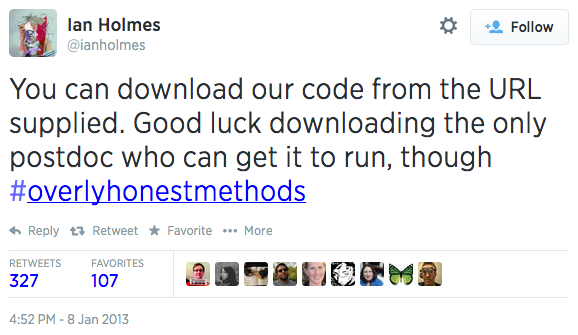
\includegraphics[width=\columnwidth]{overlyhonesttweet.png}
\caption{An \#overlyhonestmethod\newline [source: \url{https://twitter.com/ianholmes/status/288689712636493824}]}
\label{fig:overlyhonestmethod} 
\end{figure}

Ian Holmes's tweet is funny because it is so true. Often, the tool
that the paper describes doesn't exist for download. Or runs only on
one particular platform. Or might run for the author, for a while, but
will bot-rot so soon that even the author cannot compile it in two
months time.

Providing the source code of the tool helps with this, of course. But
you must also provide details of \emph{how} you built and wrote the
software:
%
you should provide the compiler and build toolchain; 
%
you should provide builds tools/makefiles/ant/etc and build instructions; 
%
you should list or link to all non-standard packages and libraries that you use; 
%
you should note the hardware and OS used. 
%
This sounds like a lot of work, but github APIs, CI, VMs and cloud can
make it easier; see Section~\ref{sec:Conclusion} at the end for more
on this.


\section{Form over function}

develop standard file formats which appropriately constrain the
models. Example: qualitative networks and Boolean networks are
standard types of biological formal
model~\cite{Kauffman1969,Schaub2007}. They can be expressed in SMV,
but this means that standard behaviours have to be hard coded for each
variable, introducing the possibility for errors. In the
BioModelAnalyzer~\cite{Benque2012}, the XML contains \emph{only} the
modifiable parameters limiting the possibility for error.


\section{9.63s} 

The benchmarks the tool describes are fashioned only for this instance
of this time. They might claim to be from the Windows device driver
set, but the reality is that they are are stripped down versions of
the originals. Stripped down so much as to be useless to anyone but
the author vs. the referee. It's worst than that really: enough
benchmarks are included to beat other tools. The comparisons are never
fair. (Neither are other peoples' comparisons against your tool.) If
every paper has to be novel, then every benchmark, too, will be novel;
there is no monotonic, historical truth in new, syntheticly-crafted
benchmarks.

It's as if, in order to beat Usain Bolt's time, you put him in a muddy
icy track, and weighed him down with 50k of excess weight. Given this
set up, you could hope to beat his 9.63s on a shorter length track.

Benchmarks should be public. They should allow anyone to contribute,
implying that the tests are in a standard format. Further, these
benchmarks must be heavily curated. Every test/assertion should be
justified. Papers should be penalized if they don't use these public
benchmarks.

A good example of some of these points is the protein data bank
(\url{http://www.pdb.org}) and Systems Biology Markup
Language~\cite{Hucka2003,Chaouiya2013}. The software ones we know of,
the SMT Competition and the SV-COMP ones~\cite{SMTComp2014,
  SVCOMP2015}, are on that journey. Such repositories would
allow the tests to be taken and easily analysed by any competitor
tool.

\section{Welcome to the Web 2.0, guys; you're 10 years late} 

you could include an interface to the tool and a model in the web
version of the paper, to demonstrate how it works i.e. make the paper
``executable''. This would allow users who are not able to install
necessary dependecies etc. to explore the model \cite{Hall2014}

Virtual machines could make testing of scaling properties more simple. 
Build a cluster of slow nodes in the cloud to demonstrate how well the
software scales for parallel calculations
%
Solves the problem of a third party not being able to test at
scale. Say because they don't have the resources to run massive HPC
compute engines.


\section{Conclusion}
\label{sec:Conclusion} 

Bringn all of the above together into an open, always-active (so always working) CI
system for tools. 

main proposal: automatic online dependency/build/traffic light system
with github hooks?

more main proposal: a lineage of the software (history/branches) and a
(more limited) lineage of the algorithm its built on




% trigger a \newpage just before the given reference
% number - used to balance the columns on the last page
% adjust value as needed - may need to be readjusted if
% the document is modified later
%\IEEEtriggeratref{37}
% The "triggered" command can be changed if desired:
%\IEEEtriggercmd{\enlargethispage{-5in}}

% BibTeX users
\bibliographystyle{IEEEtran}      % basic style, author-year citations
\bibliography{wssspe2}   % name your BibTeX data base

\end{document}
